\chapter{Baby Steps with Android}

\section{Aims}
\paragraph{} At the end of the practical portion of this topic you will be able to:

\begin{itemize}
\item Understand the basic relationship between Android project files
\item Display text using an Android View
\item Display buttons and respond when they are used
\item Display notifications (Toasts) to users
\item Log output from your app and view it using logcat
\end{itemize}

\section{Preliminaries}
\paragraph{} Create a new Android project using the process we followed for HelloAndroid. You should give your project a different name, for example, `HelloString' (because to begin with we shall be manipulating the strings that say Hello ;). It is a good idea to come up with a naming scheme for your Android projects or perhaps to organise them in folders based upon module topic or semester week number so that later in the course you can refer back to earlier code you have developed.

\paragraph{} In Android Studio open the Activity Java file. This should be called `MainActivity.java' and will be located in the 
\begin{framed}
src/uk/ac/napier/napier-id/HelloString/ 
\end{framed}
\paragraph{} folder of your project. 

\paragraph{} There isn’t a lot to see here. Most of what you see is commonly called `boilerplate' and is basically setting up the things that the Android libraries need to provide the framework for an empty project. What you will notice is that the things you see on screen when you run this app are not anywhere to be found in this Java file. This is because all the text, graphics, and layout information is created and stored in separate XML files. These XML files are then referenced from the Java code or other XML files. This means that Android has a very flexible development system which encourages well structured and reusable designs but the drawback is that it is a little complicated to get started with.

\paragraph{} There are a few things to take particular note of in the MainActivity.java file.

\begin{lstlisting}
    public class MainActivity extends Activity {
\end{lstlisting}

\paragraph{} In this line we are creating a class, called MainActivity, which inherits from the Activity parent class. Rather than creating a main method like we do in a Java program we are allowing the Android libraries to provide the main method instead. This is because we are not writing a Java program, we are writing an Android app, and these are different things. When we write an Android app we will be working within the framework of classes and libraries provided by the Android platform and there are certain requirements for an Android app to become an Android app. Because the core of an Android app is the Activity we must use the existing Android classes that provide Activity functionality. There are a number of Activity and other classes that we can inherit functionality from but for the moment we will concentrate on the core Activity class.

\paragraph{} Because we have inherited from the Activity base-class we must implement a number of methods that allow our apps functionality to `hook in' to the framework provided by the Android platform. Importantly right now we override the onCreate method. This is the method that pretty much starts the life-cycle of our app. It is called when our app is created and does a lot of work for us. In this case, with our basic HelloString app all it does is call the parent class onCreate method to ensure that the hierarchy of Activity classes are properly initialised then

\begin{lstlisting}
setContentView(R.layout.activity_main);
\end{lstlisting}

\paragraph{} Let's unpack this a little. The setContentView part is a call to a method related to displaying something on screen. We then have the argument to this method which contains 
\begin{framed}
R.layout.activity\_main
\end{framed}
\paragraph{} What this means is that we are referencing an Android resource. `R' is short for resource, notice that in package explore there is a folder called `res'. This contains all of the information about things that our can display, amongst other things. For our purposes we can consider `R' to refer to these resources. In reality it is slightly more complicated because when we build our app the contents of the res folder are assembled into a more efficient representation and the `R' file is essentially an index to our efficient representation of our resources. Going back to our line of code, without the res folder there is a sub-folder called layout, inside of which is a file called `activity\_main.xml'. This line of code is essentially saying display the layout described in activity\_main.xml, so perhaps we should take a look at that file. Use package explorer to open it.

\paragraph{} There is a lot to take in in this file. For a start. it doesn't look like a Java language source file. That is because it isn't. It is an eXtensible Markup Language (XML) file\footnote{\url{http://en.wikipedia.org/wiki/XML}}. XML is used to describe and specify Android resources. There are a number of things happening in this file. The top part

\begin{lstlisting}<RelativeLayout xmlns:android="http://schemas.android.com/apk/res/android"
    xmlns:tools="http://schemas.android.com/tools" android:layout_width="match_parent"
    android:layout_height="match_parent" android:paddingLeft="@dimen/activity_horizontal_margin"
    android:paddingRight="@dimen/activity_horizontal_margin"
    android:paddingTop="@dimen/activity_vertical_margin"
    android:paddingBottom="@dimen/activity_vertical_margin" tools:context=".MainActivity">
\end{lstlisting}

\paragraph{} basically describes a layout for the things to display on screen. Essentially telling Android to use the `Relative Layout' to organise the things that it draws and to use the parameters that are supplied e.g. layout\_height, paddingRight, paddingTop, and paddingBottom. We will see more about layouts and how to arrange things nicely on screen in the next practical so for now we will just ignore it. The next section is more interesting right now:

\begin{lstlisting}    <TextView android:text="@string/hello_world" android:layout_width="wrap_content"
        android:layout_height="wrap_content" />
\end{lstlisting}

\paragraph{} This is interesting because it is the bit that tells the Android platform to display our "Hello World" message. Again, like the use of `R' in MainActivity.java to provide flexibility we have another bit of indirection. Instead of just having all of the strings that our app uses in the place that they are used, instead we have them all collected in a single location, another resource file, called strings.xml which can be found here

\begin{framed}
res/values/strings.xml
\end{framed}

\paragraph{} {\bf{Why do you think that it might be useful to collect all of the strings together in one place?}}

\paragraph{} Our layout file contains a reference to a specific string, stored in the strings.xml resource file, which we want to be displayed onscreen in this layout. The reference is the `@string/hello\_world'. The reference uses `@string' to indicate that the string resource is in the strings.xml file then the name of the resource `hello\_world' to specify the particular string to display. Use package explorer to find and open the strings.xml file.

\begin{lstlisting}
<?xml version="1.0" encoding="utf-8"?>
<resources>

    <string name="app_name">HelloAndroid</string>
    <string name="hello_world">Hello world!</string>
    <string name="action_settings">Settings</string>

</resources>
\end{lstlisting}

\paragraph{} The string that displays the message is the one called `hello\_world'. The content of the string comes between the $<$string name="..."$>$$<$/string$>$ tags, in this cases ``Hello world!''. If you havn't done so yet. Run the project and look at the output. Then try altering the content of the string to display another message of your own design. From here you can even change the name of your app by altering the content of the `app\_name' string but we can leave that alone for now.

\paragraph{} While we have the emulator running we will try using it a bit more, the advanced features of the emulator and how we can interface with it will be covered in a later practical but you should make yourself familiar with what the various buttons on the emulator can do:
•	the home button will return you to the home screen, 
•	the menu button differs with each application and 
•	the back button acts like a browser back button. You will find that the emulator contains the majority of a basic Android phones features, exceptions include Bluetooth and camera as they would require specific hardware.
It is possible to run applications already on the emulator, including our application from earlier. Click the launcher grid button (in the centre of the home screen) and scroll through the list of existing apps, you should be able to find your app and run it from here. To add an app to the home page, press and hold the icon and when the emulator changes to the home page you can drag the icon into place and release it to place it there.

\begin{figure}[H]%[htb]
\centering
    \begin{subfigure}[b]{0.45\textwidth}
        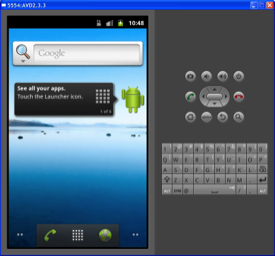
\includegraphics[width=\textwidth]{images/android_home}
        \caption{Android Home}
        \label{fig:android-home}
    \end{subfigure}
    ~ 
    \begin{subfigure}[b]{0.45\textwidth}
        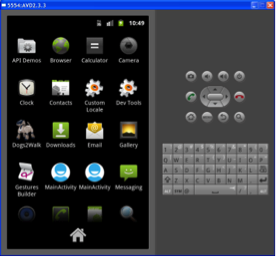
\includegraphics[width=\textwidth]{images/android_apps}
        \caption{Android Apps}
        \label{fig:android-apps}
    \end{subfigure}
\caption{Android home screen \& apps}
\label{fig:android-home-apps}
\end{figure}

\section{The DateTime App}
\paragraph{}Now we have an understanding of how the applications are built and executed on the emulator we will build our first application that does something more than just display the Hello message. Along the way we will explore some of the basic user interface controls available on the Android platform. On Android anything that can be displayed on screen is called a View and this includes all of those elements that we are used to on other platforms that we usually refer to as GUI widgets.

\paragraph{} We're going to create an app which displays the current date and time when you click a button. Create a new app and call it `DateTime'. Open the graphical layout - one way of doing this is simply to double click the activity\_main.xml file in the res/layout folder. You can delete the HelloWorld message, just select it with the mouse and delete it, as we won't be using it.

You should see an area of the Android Studio UI which provides a `Palette' or `toolbox' of graphical widgets that you can use in your app. Drag a textview view from the palette onto the AndroidApp activity layout. Notice that the graphical layout is a good way to place and arrange Android views on screen to rapidly create a GUI. Select the new Text View – then change the Text property to ``DateTime'' (without the quotes) and the name to ``TextView1''. Click now on the activity\_main.xml tab to see what has happened to the XML code – you should now have a block called $<$EditText...$>$ like so

\begin{lstlisting}
<TextView
        android:layout_width="wrap_content"
        android:layout_height="wrap_content"
        android:text="DateTime"
        android:id="@+id/textView1"
        android:layout_below="@+id/button1"
        android:layout_centerHorizontal="true" />
\end{lstlisting}

\paragraph{} Now return to graphical layout and select Form Widgets. Drag a button over to your activity layout.  Right click (or double click in Android Studio) to edit the text that goes onto the button - and select Edit Text. You can enter the new text in the field at the bottom (under New String...). Change to ``Click me!''. The default name for your button is button1 – check this by clicking on the button then looking at the properties.

\begin{lstlisting}
<Button
        android:layout_width="wrap_content"
        android:layout_height="wrap_content"
        android:text="Click Me!"
        android:id="@+id/button1"
        android:layout_centerHorizontal="true"
        android:layout_marginTop="79dp"
        android:layout_centerVertical="true" />
\end{lstlisting}

\paragraph{} So we now have a text box and we have a button. Check your app now – select the project from the Package Explorer then click the play button (a green `play' triangle on the menu bar):

\paragraph{} The problem now is that our app doesn't actually do anything. The Click Me! button has no functionality and the TextView will just display DateTime forever. We need to write some code to do something when the button is clicked. We’re going to overwrite the DateTime string with the actual date and time. How are we going to do this? Well, we need to have a handler that will listen for button clicks, we need to write a little bit of code to get the current time and date, and we need a little bit of code to update the TextView with our new time and date.

\paragraph{} Open MainActivity.java. First we need to add some imports so that our app can access the libraries that it needs to do our extra functionality. By default the basic app project only has the minimal set of imports that it needs to display the Hello World message. We have to add other imports to do different things. These are the imports that we need in MainActivity.java in addition to the ones that are already there:

\begin{lstlisting}
import android.view.View;
import android.view.View.OnClickListener;
import android.widget.Button;
import android.widget.TextView;
import java.util.Date;
\end{lstlisting}

\paragraph{} Now we need to add some code to the onCreate method:

\begin{lstlisting}
Button btn1 = (Button) findViewById(R.id.button1);
        btn1.setOnClickListener(new OnClickListener() {
            @Override
            public void onClick(View v) {
                TextView tv1 = (TextView) findViewById(R.id.textView1);
                tv1.setText(new Date().toString());
            }
        });
\end{lstlisting}

\paragraph{} You should now be able to run your app and each time you click the button you will see an updated date and time displayed in the TextView.

\paragraph{} Just for completion. Open the strings.xml file for your app and add a new string resource to represent the text of your button, e.g.

\begin{lstlisting}
<string name="button1">Click Me!</string>
\end{lstlisting}

\paragraph{} Now, in your activity\_main.xml, update the entry for the button to reference the string resource rather than embedding the string directly in the activity, e.g.

\begin{lstlisting}
android:text="@string/button1"
\end{lstlisting}

\paragraph{} Now try to do the same for the TextView. Add a string resource for the default content of the TextView then reference that string resource from activity\_main.xml

\paragraph{} You should now experiment with the various settings that you can use for TextViews and Buttons. Try adding a text view or more buttons and changing the text on them rather than the text on the button being pressed. Use the graphical designer to drag and drop various views onto your activity and use the property inspector to set various properties for the views. Remember to frequently run your app after you have made even small changes to see what effect they have. You should also frequently compare the visual view of the activity which gives you an idea of how the app will look with the contents of the activities XML file. The aim of this is to get a feel for the various widgets that are available, the settings that they can have, and how the views are actually represented as resources in the XML files of your app.

\section{Toasts}
\paragraph{} A toast\footnote{There is more general information about Toasts available at the Android website \url{http://developer.android.com/guide/topics/ui/notifiers/toasts.html} as wells developer documentation \url{developer.android.com/reference/android/widget/Toast.html}} is a view that contains a quick message or notification to the user, the Toast class helps you create and show Toast messages without having to set up the View in a layout file. When the View is shown to the user it appears to float over the current application activity, it never receives focus over and it will not interrupt the users current actions like typing. Examples of common Toast messages are the volume control or save messages when you save a draft of a text message. The idea is to be as unobtrusive as possible while showing important information to the user.

\paragraph{} We can adapt our DateTime app to display a toast each time we click the button. This will illustrate how you can integrate toasts into your own apps. In MainActivity.java we need an import for the Toasts class:

\begin{lstlisting}
import android.widget.Toast;
\end{lstlisting}

\paragraph{} Having imported the Toast class we can use it, which is pretty straightforward. In the onClick handler that we created earlier for our button, just add the following after the call to setText on our TextView

\begin{lstlisting}
Toast.makeText(MainActivity.this, tv1.getText(),Toast.LENGTH_LONG).show();
\end{lstlisting}

\paragraph{} Toasts are also a useful way to do quick output if you want to just check the value of something during development. However there is also a much better way....

\section{Logging}
\paragraph{} Logging\footnote{Developer documentaiton available here \url{http://developer.android.com/reference/android/util/Log.html}} is really important once you start to build larger apps. Because Android doesn't have a console or terminal which our app can output messages to we need something else. We could add widgets into our GUI to let us quickly see the values that our apps hold but this is far from ideal. The logging subsystem is designed to enable you to output data from your app outside of the graphcial views that make up your app.

\paragraph{} Android Studio has areas set aside to display logs whilst you are developing and running your apps. These are in the logcat area and will display both log messages that you cause to be sent from your code, as well as log messages that arise due to errors during runtime.

\paragraph{} To use logging we need some imports again in MainActivity.java

\begin{lstlisting}
import android.util.Log;
\end{lstlisting}

then to cause a line to be written to the log we just need a line like the following (place it in the onClick listener for your button to try it out):

\begin{lstlisting}
Log.i("org.simonwells.datetime","Button pressed");
\end{lstlisting}

\paragraph{} Notice that there are two arguments, the first is our namespace, which you should have set to match either your personal domain name, if you have one, or something like `uk.ac.napier.xx1234' if you created one based on your Napier ID. The second argument is the actual string to write into the log. You could write a static string here as we have done above with `Button pressed' or else you can build the string to display, e.g. including the id of the concerned view so that you can identify exactly which view caused the log line to be created. This is especially useful as your apps get bigger and involve more views (and more things that could go wrong).

\paragraph{} When you run your app and press the button you should see a line similar to the following in logcat:

\begin{framed}
{\scriptsize{
01-21 14:29:21.654 23977-23977/org.simonwells.datetime I/org.simonwells.datetime: Button pressed
}}
\end{framed}

\section{Summary}
\paragraph{} In this practical we have 

\begin{itemize}
\item Investigated the relationship between Android project files made up of Java source files, XML files and others.
\item Displayed text using an Android View
\item Displayed buttons and responded when they have been used
\item Displayed notifications (Toasts) to users
\item Logged output from our apps and viewed it using logcat
\end{itemize}

